\chapter{Representação de dados}
\label{cap:representacaodedados}

\begin{chapquote}{Autor desconhecido}
``Existem 10 tipos de pessoas no mundo;
aquelas que entendem binário e aquelas que
não entendem binário.''
\end{chapquote}

A representação de dados se refere a como as informações são armazenadas no computador. Existe um método específico para armazenar números inteiros que é diferente do armazenamento de valores de ponto flutuante, que é diferente do armazenamento de caracteres. Este capítulo apresenta um breve resumo dos esquemas de representação de inteiro, ponto flutuante e ASCII.

Presume-se que o leitor já esteja familiarizado com os sistemas de numeração binária, decimal e hexadecimal.

Deve-se observar que, se não for especificado, um número está na base 10. Além disso, um número precedido por 0x é um valor hexadecimal. Por exemplo, $ 19 = 19_{10}  = 13_{16} = 0x13$.

\section{Representação de Inteiros}
Representar números inteiros refere-se a como o computador armazena ou representa um número na memória. O computador representa números em binários (1's e 0's). No entanto, o computador tem uma quantidade limitada de espaço que pode ser usada para cada número ou variável.
Isso afeta diretamente o tamanho, ou intervalo, do número que pode ser representado. Por exemplo, um byte (8 bits) pode ser usado para representar $ 2^8 $ ou $ 256 $ números diferentes. Esses 256 números diferentes podem não ter sinal (todos positivos), caso em que podemos representar qualquer número entre 0 e 255 (inclusive). Se escolhermos sinais (valores positivos e negativos), podemos representar qualquer número entre $ -128 $ e $ +127 $ (inclusive).

Se esse intervalo não for grande o suficiente para lidar com os valores pretendidos, um tamanho maior deve ser usado. Por exemplo, uma palavra (16 bits) pode ser usada para representar $ 2^{16} $ ou 65.536 valores diferentes, e uma palavra dupla (32 bits) pode ser usada para representar $ 2^{32} $ ou 4.294.967.296 números diferentes. Portanto, se você quiser armazenar um valor de 100.000, será necessária uma palavra dupla.

Como você deve se lembrar de C, C++ ou Java, uma declaração de número inteiro (por exemplo, \textbf{int} \textbf{<variável>}) é uma única palavra dupla que pode ser usada para representar valores entre
 $ -2^{31} $ 
 ($-2.147.483.648$) e 
 $ +2^{31} - 1 $
  ($+ 2.147.483.647$).

A Tabela \ref{tab:faixas} mostra os intervalos associados aos tamanhos típicos:

\begin{table}[h]
	\centering
	\small
	\begin{tabular}{|l|c|c|c|}
		\hline
		\rowcolor[HTML]{C0C0C0} 
		\textbf{Tamanho} & \textbf{Tamanho} & \textbf{Faixa sem sinal} & \textbf{Faixa sinalizada} \\ \hline
		Bytes (8-bits) & $2^8$ & 0 a 255 & $-128$ a $+127$\\ \hline
		Words (16-bits) & $2^{16}$ & 0 a 65.535 & $-32768$ a $+32767$\\ \hline
		Double-words (32-bits) & $2^{32}$ & 0 a 4.294.967.295 & $-^2.147.483.648$ a\\
		&&& $+2.147.483.647$\\ \hline
		Quadword & $2^{64}$ & 0 a $2^{64}-1$ & $-2^{63}$ a $2^{63}-1$\\ \hline
		Double quadword & $2^{128}$ & 0 a 255 & $-128$ a $+127$\\ \hline
	\end{tabular}
	
	\caption{Faixas de valores para tamanhos típicos.}
	\label{tab:faixas}
\end{table}

Para determinar se um valor pode ser representado, você precisará saber o tamanho do elemento de armazenamento (byte, palavra, palavra dupla, palavra quádrupla, etc.) sendo usado e se os valores são sinalizados ou não.

\begin{itemize}
	\item Para representar valores \textit{não sinalizados} dentro do intervalo de um determinado tamanho de armazenamento, o binário padrão é usado. 
	\item Para representar \textit{valores com sinais} dentro do intervalo, o complemento a dois é usado. Especificamente, o processo de codificação de complemento a dois se aplica aos valores na faixa negativa. Para valores dentro da faixa positiva, o binário padrão é usado.
\end{itemize}

Por exemplo, o intervalo de bytes não sinalizados pode ser representado usando uma linha numérica da seguinte maneira:

\vspace{5mm}
\begin{tikzpicture}
\draw[white, thick, |-] (-2.95,0) -- (0,0)  node [black, below=2pt]
{0};
\draw[blue, thick,|-] (0,0) -- (2.5,0);
\draw[blue, thick,|-|] (2.5,0) -- (5,0) node [black, below=2pt]
{255};
\end{tikzpicture}

Por exemplo, o intervalo de bytes sinalizados também pode ser representado usando uma linha numérica da seguinte forma:

\vspace{5mm}
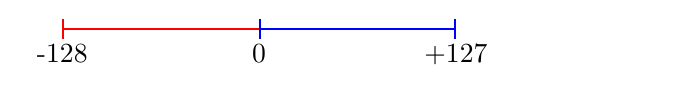
\begin{tikzpicture}
\draw[red, thick, |-]  (-2.5,0) node [black, below=2pt]
{-128} -- (0,0)  node [black, below=2pt]
{0};
\draw[blue, thick,|-|]  (0,0)  -- (2.5,0) node [black, below=2pt]
{+127};
\draw[white, thick,|-|] (2.5,0) -- (5,0);
\end{tikzpicture}

O mesmo conceito se aplica a meias palavras e palavras que possuem intervalos maiores.


Como os valores sem sinal têm um intervalo diferente, apenas positivo, do que os valores com sinal, há sobreposição entre os valores. Isso pode ser muito confuso ao examinar variáveis na memória (com o depurador).

Por exemplo, quando os valores sem sinal e com sinal estão dentro do intervalo positivo de sobreposição (0 a +127):

\begin{itemize}
	\item Uma representação de byte com sinal de $ 12_{10} $ é $ 0x0C_{16} $
	\item Uma representação de byte sem sinal de $-12_{10} $ também é $ 0x0C_{16} $
\end{itemize}

Quando os valores não sinalizados e sinalizados estão fora do intervalo de sobreposição:
\begin{itemize}
	\item Uma representação de byte sinalizado de $ -15_{10} $ é $ 0xF1_{16} $
	\item Uma representação de byte não sinalizado de $ 241_{10} $ também é $ 0xF1_{`} $
\end{itemize}

Essa sobreposição pode causar confusão, a menos que os tipos de dados sejam definidos de forma clara e correta.

\subsection{Complemento a Dois}
A seguir é descrito como encontrar a representação de complemento a dois para valores negativos (valores não positivos).

Para pegar o complemento a dois de um número:
\begin{enumerate}
	\item pegue o complemento a um (negar)
	\item adicione 1 (em binário)
\end{enumerate}

O mesmo processo é usado para codificar um valor decimal no complemento a dois e do complemento a dois de volta ao decimal. As seções a seguir fornecem alguns exemplos.

\subsubsection{Exemplo de Byte}
Por exemplo, para encontrar a representação com tamanho de byte (8 bits), do complemento a dois de $ -9 $ e $ -12$.

\begin{minipage}{.5\textwidth}
\begin{tabular}{|r|c|}
	\hline
	$ 9 (8+1)= $ & 0000 1001\\ \hline
	Passo 1 & 1111 0110\\ \hline
	Passo 2 & 1111 0111\\ \hline
	-9 (em hexa) & \textbf{F7}\\ \hline
\end{tabular}
	
\end{minipage} 
\begin{minipage}{.5\textwidth}
\begin{tabular}{|r|c|}
	\hline
	$ 12 (8+4)= $ & 0000 1100\\ \hline
	Passo 1 & 1111 0011\\ \hline
	Passo 2 & 1111 0100\\ \hline
	-12 (em hexa) & \textbf{F4}\\ \hline
\end{tabular}
	
\end{minipage}%

\vspace{5mm}

Observe que todos os bits para o tamanho fornecido, byte neste exemplo, devem ser especificados.

\subsubsection{Exemplo de Word}
Para encontrar o tamanho da palavra (16 bits), a representação em complemento a dois de $ -18 $ e $ -40$.

\begin{minipage}{.5\textwidth}
	\begin{tabular}{|r|c|}
		\hline
		$ 18 (6+2)= $ & 0000000000010010\\ \hline
		Passo 1 & 1111111111101101\\ \hline
		Passo 2 & 1111111111101110\\ \hline
		-9 (em hexa) & \textbf{FFEE}\\ \hline
	\end{tabular}
	
\end{minipage} 
\begin{minipage}{.5\textwidth}
	\begin{tabular}{|r|c|}
		\hline
		$ 40 (32+8)= $ & 0000000000101000\\ \hline
		Passo 1 & 1111111111010111\\ \hline
		Passo 2 & 1111111111011000\\ \hline
		-12 (em hexa) & \textbf{FFD8}\\ \hline
	\end{tabular}
	
\end{minipage}%

\vspace{5mm}
Observe que todos os bits para o tamanho fornecido, palavras nesses exemplos, devem ser especificados.

\section{Adição não sinalizada e sinalizada}
Conforme observado anteriormente, as representações não assinadas e assinadas podem fornecer diferentes interpretações para o valor final sendo representado. No entanto, as operações de adição e subtração são as mesmas. Por exemplo:

\begin{minipage}{.5\textwidth}
	\begin{tabular}{|r|c|}
		\hline
		$ 241 $ & 11110001\\ \hline
		$+7$ & 00000111\\ \specialrule{2.5pt}{1pt}{1pt}
		$ 248 $ & 11111000\\ \specialrule{2.5pt}{1pt}{1pt}
		$ 248 $ = & \textbf{F8}\\ \hline
	\end{tabular}
	
\end{minipage} 
\begin{minipage}{.5\textwidth}
	\begin{tabular}{|r|c|}
		\hline
		$ -15 $ & 11110001\\ \hline
		$+7$ & 00000111\\ \specialrule{2.5pt}{1pt}{1pt}
		$ -8 $& 11111000\\ \specialrule{2.5pt}{1pt}{1pt}
		$ -8 = $ & \textbf{F8}\\ \hline
	\end{tabular}
	
\end{minipage}%

\vspace{5mm}

O resultado final de \textbf{0xF8} pode ser interpretado como 248 para representação não sinalizada e $ -8 $ para uma representação sinalizada. Além disso, $ 0xF8_{16} $ é o $^{\circ}$ (símbolo de grau) na tabela ASCII.

Como tal, é muito importante ter uma definição clara dos tamanhos (byte, meia palavra, palavra, etc.) e tipos (com ou sem sinal) de dados para as operações que estão sendo realizadas.

\section{Representação de ponto flutuante}
Os problemas de representação para números de ponto flutuante são mais complexos. Há uma série de representações de ponto flutuante para vários intervalos de valor. Para simplificar, examinaremos principalmente o padrão de ponto flutuante \textbf{IEEE 754} de 32 bits.

\subsection{Representação IEEE de 32 bits}
O padrão de ponto flutuante\textbf{ IEEE 754} de 32 bits é definido da seguinte forma:

\noindent
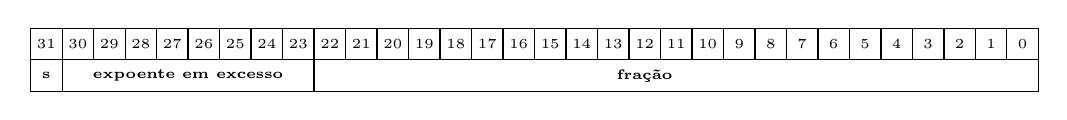
\begin{tikzpicture}[scale=0.4]
\foreach \x in {31,...,0}
{
	\draw (\x,0) +(-.5,-.5) rectangle ++(.5,.5);
	\draw (31-\x, 0) node{{\tiny \x}};	
}
\draw(0,-1) +(-.5,-.5) rectangle ++(.5,.5);
\draw(1,-1) +(-.5,-.5) rectangle ++(7.5,.5);
\draw(9,-1) +(-.5,-.5) rectangle ++(22.5,.5);
\draw(0, -1) node{{\tiny \textbf{s}}};
\draw(4.5, -1) node{{\tiny \textbf{expoente em excesso}}};
\draw(19, -1) node{{\tiny \textbf{fração}}};

\end{tikzpicture}

Onde \textbf{s} é o sinal (0 $\Rightarrow $ positivo e 1 $ \Rightarrow $  negativo). Mais formalmente, isso pode ser escrito como:
\begin{center}
	$ N = (-1)^S \times 1.F \times 2^{E-127} $
\end{center}

Ao representar valores de ponto flutuante, a primeira etapa é converter o valor de ponto flutuante em binário. A tabela a seguir fornece um breve lembrete de como o binário lida com componentes fracionários:

\vspace{5mm}
\begin{center}
	\begin{tabular}{|c|c|c|c|c|c|c|c|c|c|}
	\hline
	         &$2^3$& $2^2$ & $2^1$ & $2^0$ & & $2^{-1}$  & $2^{-2}$ & $2^{-3}$ & \\ \hline
	$\ldots$ & 8   & 4     & 2     & 1     &.& 1/2       &  1/4     & 1/8 & $\ldots$\\ \hline
	         & 0   & 0     & 0     & 0     &.& 0         &  0     & 0 & \\ \hline
\end{tabular}
\end{center}
\vspace{5mm}

Por exemplo, $ 100,101_2 $ seria $ 4,625_{10} $. Para decimais repetidas, o cálculo do valor binário pode ser demorado. No entanto, há um limite, pois os computadores têm tamanhos de armazenamento finitos (32 bits neste exemplo).

A próxima etapa é mostrar o valor em notação científica normalizada em binário. Isso significa que o número deve ter um único dígito inicial diferente de zero à esquerda da vírgula decimal. Por exemplo, $ 8,125_{10} $ é $ 1000,001_2 $ (ou $ 1000,001_2 \times 2^0$) e em notação científica binária normalizada que seria escrita como $ 1,000001 \times 2^3 $ (já que a vírgula decimal foi movida três casas para a esquerda). Claro, se o número fosse $ 0,125_{10} $, o binário seria $ 0,001_2 $ (ou $ 0,001_2 \times 2^0 $) e a notação científica normalizada seria $ 1,0 \times 2_{-3} $ (já que a vírgula decimal foi movida três casas para a direita). Os números após o 1 inicial, não incluindo o 1 inicial, são armazenados justificados à esquerda na parte da fração da palavra dupla.

A próxima etapa é calcular o expoente em excesso, que é o expoente da notação científica normalizada com mais o excesso. O excesso para o padrão de ponto flutuante de 32 bits \textbf{IEEE 754} é $ 127_{10} $. O resultado deve ser convertido para um byte (8 bits) e armazenado na parte expoente em excesso da palavra.

Observe que a conversão da representação de ponto flutuante de 32 bits \textbf{IEEE 754} para o valor decimal é feita ao contrário, no entanto, o 1 inicial deve ser adicionado de volta (já que não é armazenado na palavra). Além disso, o excesso é subtraído (em vez de adicionada).

\subsubsection{Exemplos de representação IEEE de 32 bits}
Esta seção apresenta vários exemplos de codificação e decodificação de representação de ponto flutuante para referência.

\subsubsection{Exemplo: $-7.75_{10} $ }
Por exemplo, para encontrar a representação de ponto flutuante IEEE 754 de 32 bits para $-7.75_{10} $: 

\begin{tabular}{lll}
	1. Determinar o sinal: & $ -7.75 \Rightarrow 1 $ (posto que negativo)\\
	2. converter para binário: & $ -7.75 = -0111.11_2 $\\
	3. notação científica normalizada: & $ =	1.1111 \times 2^2 $\\
	4. calcular expoente em excesso: & $ 2_{10} + 127_{10} = 129_{10} $\\
	e converter para binário: & $ = 10000001_2 $\\
	5. escrever componentes em binário: & \\
    \multicolumn{2}{l}{\begin{tabular}{ccl}
    		sinal & expoente & mantissa\\
    		1 & 10000001 & 11110000000000000000000\\
    \end{tabular}} \\
    \multicolumn{2}{l}{6. converter para hexadecimal (dividido em grupos de 4)} \\
    \multicolumn{2}{l}{11000000111110000000000000000000}\\
    \multicolumn{2}{l}{\begin{tabular}{*8c}
     1100 & 0000 & 1111 & 1000 & 0000 & 0000 & 0000 & 0000\\
     C    & 0    & F    & 8    & 0    & 0    & 0    & 0\\
    	\end{tabular}
    }\\
    7. resultado final: & $ C0F8 0000_16 $\\
	
\end{tabular}


